
\subsection{Action Spaces} \label{sec:action_space}

As introduced in \cref{sec:domain_view}, ACUs can utilize four main types of actions: mouse/touch and keyboard actions, direct UI access, task-tailored actions, and executable code. 
In the following, we discuss each of these action spaces, while Table~\ref{tab:interaction_literature} provides the corresponding details for each ACU.


\subsubsection{Mouse/Touch and Keyboard}\label{sec:action_space_mouse}

Mouse, touch, and keyboard actions align closely with human interaction patterns, facilitating data collection and training \citep{humphreys_data-driven_2022}.
Both mouse actions (e.g., \texttt{click(x,y)}) and touch actions (e.g., \texttt{tap(x,y)}) require \emph{absolute} screen coordinates \texttt{(x,y)}, making them conceptually identical for ACUs\footnote{For humans, mouse actions are relative (to the current cursor position) and touch actions are absolute.}.
\Cref{fig:mouse-keyboard-action} summarizes approaches for predicting screen coordinates.
Some methods make discrete predictions, by either predicting a position on a low-resolution coordinate grid \citepeg{shi_world_2017,toyama_androidenv_2021}, predicting two interdependent discrete values for the \texttt{x} and \texttt{y} coordinates \citepeg{humphreys_data-driven_2022}, or generating discrete tokens through a text generation model \citepeg{hong_cogagent_2024}. Other approaches use continuous values by predicting two interdependent continuous coordinate values \citepeg{toyama_androidenv_2021}.
It remains unclear whether one prediction strategy is universally superior; instead, the choice usually depends on the agent architecture and task.
% (e.g., LLMs naturally generate coordinate tokens) and the task at hand (e.g., continuous outputs are needed for smooth gestures like swipes, whereas low-resolution predictions are sufficient for tasks requiring limited precision).
%
\begin{figure}[t]
    \centering
    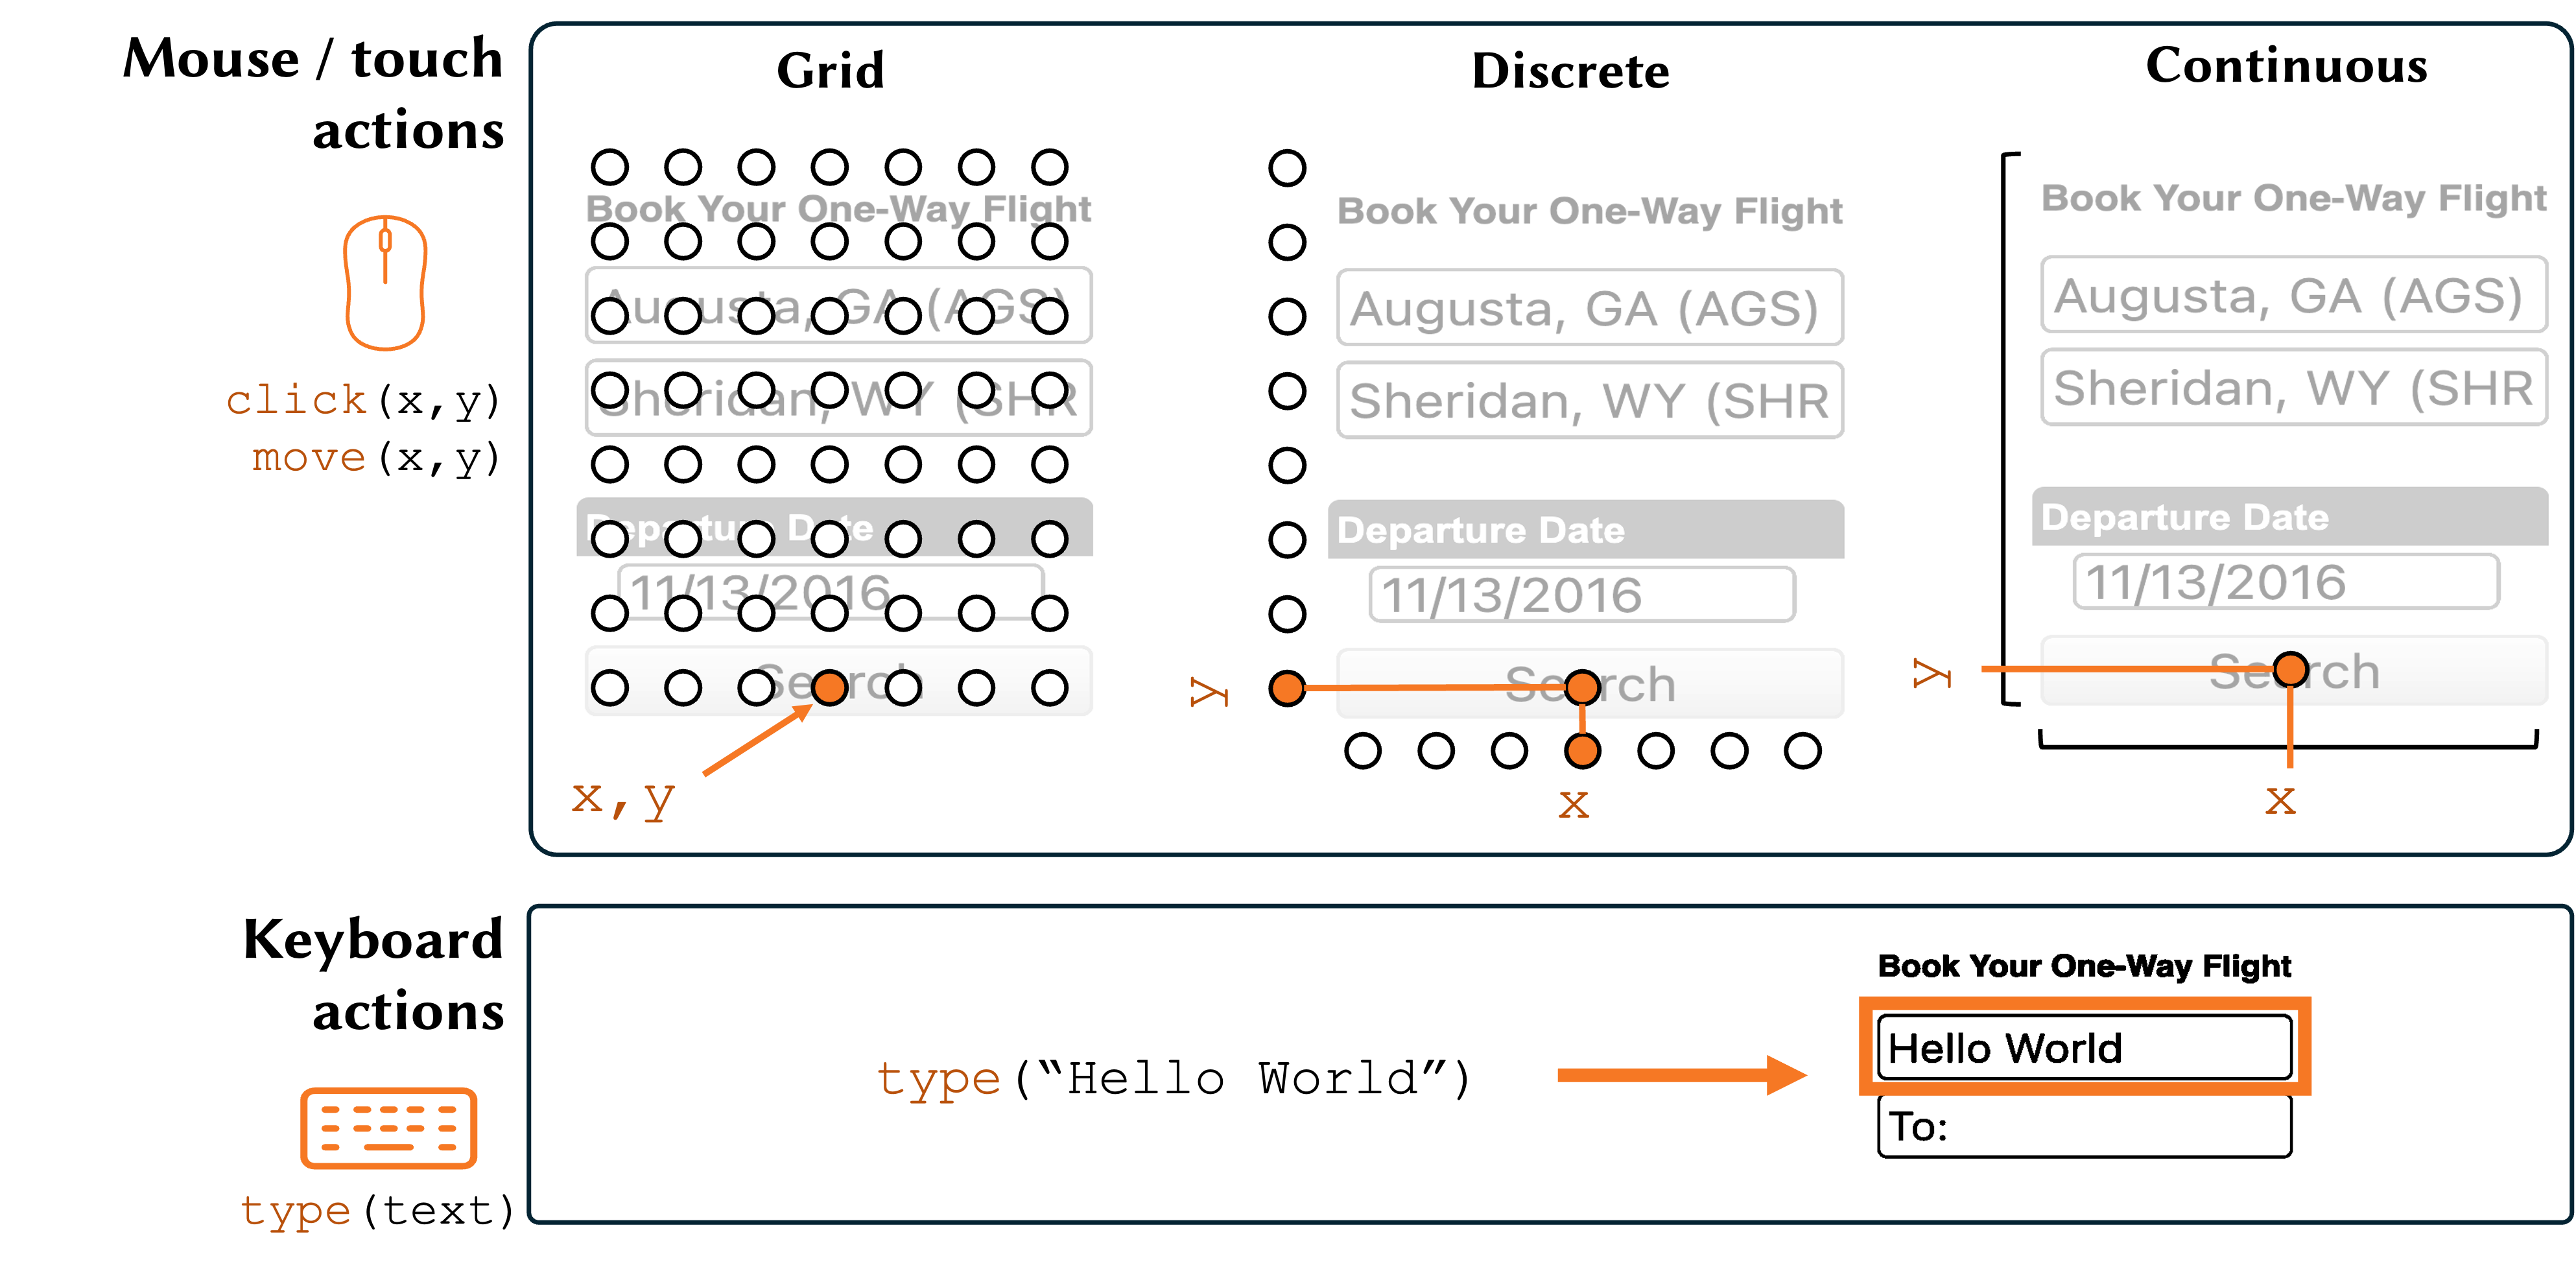
\includegraphics[width=0.65\linewidth]{figures/mouse_keyboard_action.png}
    \caption{Common mouse and keyboard actions, highlighting coordinate prediction.}
    \Description{Visualization of mouse and keyboard action modalities in agent control interfaces.
    The figure clarifies differences between common screen-coordinate prediction modes in user interface control. In the top section, three types of mouse or touch actions are shown using illustrative overlays: (1) grid-based prediction constrains clicks to fixed grid points, (2) discrete prediction allows selection from independent horizontal and vertical positions, and (3) continuous prediction enables unconstrained coordinate selection. These modes are visualized over a web form to highlight spatial precision. The bottom section shows a keyboard input scenario, where an agent types into a text box within a form interface. This comparison illustrates how action types differ in terms of input structure, spatial for mouse/touch, symbolic for keyboard, and supports the distinction between discrete and continuous action spaces.}
    \label{fig:mouse-keyboard-action}
\end{figure}

Keyboard actions (e.g., \texttt{type(text)}) are typically used to input text into a previously selected UI element.
While earlier methods relied on predefined text fragments \citepeg{humphreys_data-driven_2022} or extracted text from the instruction $i$ \citepeg{gur_learning_2019} as input, in most of the current systems, ACUs generate the text using a language model \citepeg{hong_cogagent_2024}, as this provides the required freedom to type diverse texts. 
%
% While free-text typing is a general-purpose action applicable across various applications, predicting predefined text fragments is often constrained to specific contexts and not used by general-purpose ACUs.
%
Beyond typing, keyboard actions are frequently used for special commands, such as navigating via pressing arrow keys \citepeg{li_zero-shot_2023} or using shortcuts such as \texttt{select all}, \texttt{copy}, or \texttt{paste} \citepeg{cho_caap_2024}.



\subsubsection{Direct UI Access}\label{sec:action_space_direct}

Direct UI access actions such as \texttt{click(e)} or \texttt{type(e, text)} target a specific UI element \texttt{e} observed by the agent.
Agents typically identify these elements \texttt{e} by either predicting unique identifiers like HTML \texttt{id} tags \citepeg{li_zero-shot_2023}, XPath\footnote{https://www.w3.org/TR/xpath-31/} descriptions \citep{kim_language_2023} (for an example of predicting \texttt{click(id=search)} based on \texttt{\(<\)button id="search"\(>\)} see \cref{fig:direct-action}), or by scoring and selecting from all visible elements \citepeg{jia_dom-q-net_2019, li_uinav_2024}.
%
\begin{figure}[b]
    \centering
    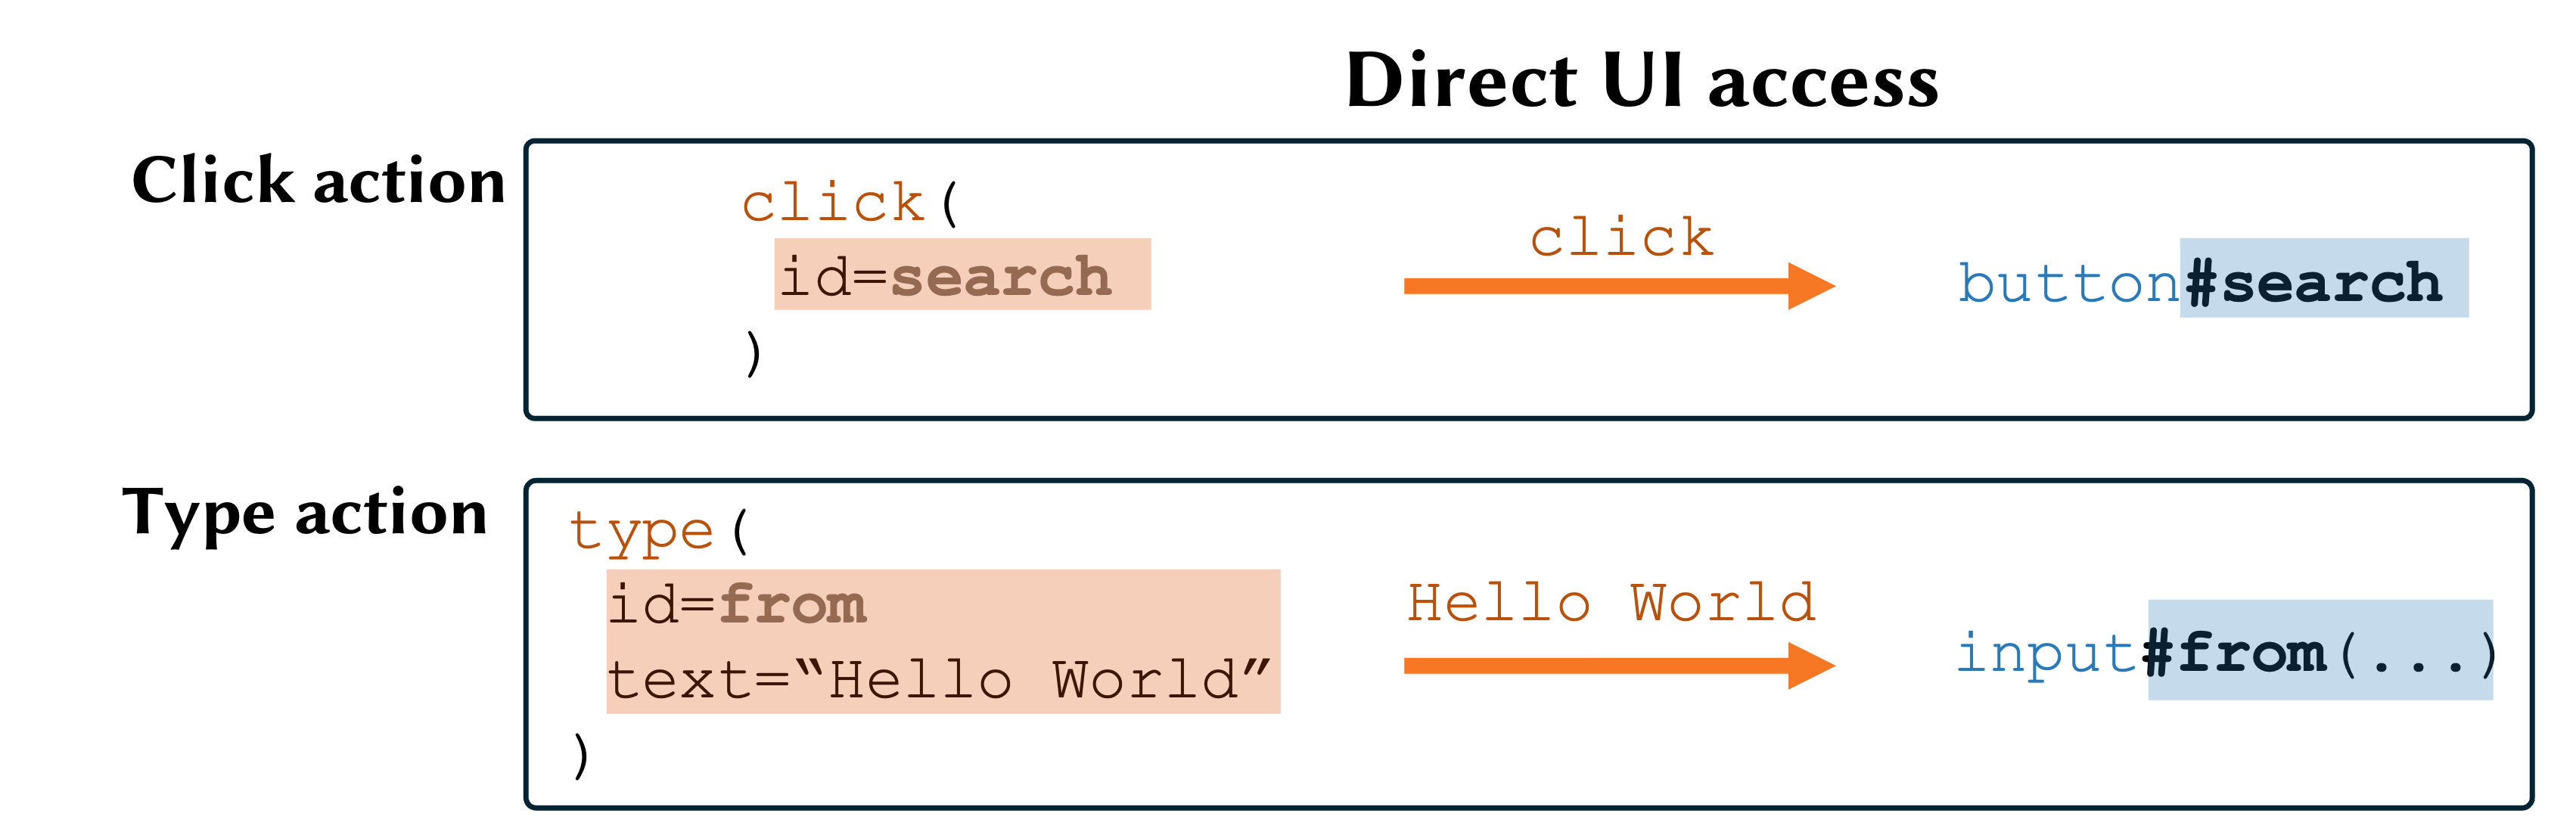
\includegraphics[width=0.6\linewidth]{figures/direct_action.png}
    \caption{Common direct UI access actions, referencing the HTML element by its \texttt{id} attribute.}
    \Description{The figure illustrates examples of direct UI access targeting HTML elements via their bolded \texttt{id} attributes. The first example demonstrates a click action where the function call specifies the \texttt{id} as ``search'' to trigger a button click. The second example shows a type action, in which the function call targets the input field with \texttt{id} equals ``form'' to enter the text ``Hello World.'' Arrows visually connect each function call to its respective HTML element, emphasizing the explicit mapping between the code and interface components.}
    \label{fig:direct-action}
\end{figure}

To simplify selection, agents may restrict referenceable elements to leaf nodes in the user interface tree \citepeg{liu_reinforcement_2018} or pre-filter them with an auxiliary model that can preselect potential candidate elements \citepeg{deng_mind2web_2023}. For specific tasks such as web navigation, agents may be limited by design to selecting hyperlinks only \citep{zaheer_learning_2022, chen_webvln_2024}.

After selecting an element, optional text input follows similar generation strategies as got keyboard input, including generating free-form text \citepeg{li_zero-shot_2023}, selecting predefined fragments \citepeg{shvo_appbuddy_2021}, or extracting text from the instruction \citepeg{jia_dom-q-net_2019}.

By classifying each reviewed ACU, we identify direct UI access as the most widely adopted action space in the literature (see Appendix~\cref{fig:action-space-dist}). We believe this dominance is due to its balance between generality and learnability. Unlike coordinate-based mouse or touch actions, which require fine-grained spatial reasoning and introduce high-dimensional prediction challenges, direct UI access operates over a lower-dimensional and semantically meaningful action space. By allowing agents to refer to structured element identifiers (e.g., \texttt{id}, XPath, or other selectors), this form of interaction abstracts away spatial complexity while still supporting a broad range of tasks.
However, as it requires an identifier for the UI elements, it is primarily compatible with text observations and, as discussed in the previous section, does therefore not scale well to the desktop domain.
Also, it typically only works well for simplified, well-structured UIs that are often not available for real-world use cases but common for earlier benchmarks (see \cref{sec:datasets}).


\subsubsection{Task-Tailored Actions}\label{sec:action_space_task}
Task-tailored actions are environment-specific commands for common operations.
For instance, \citet{wang_officebench_2024} define application-specific actions such as \texttt{create\_event} for a calendar application and \texttt{send\_email} for an email client.
These high-level actions reduce learning complexity as they typically correspond to an entire trajectory of clicking actions.
Nevertheless, the downside is that they require additional engineering as these subroutines are often hand-crafted \citepeg{wang_officebench_2024, tan_towards_2024}.

We consider most task-specific actions as a shortcut that might help to improve on narrowly designed benchmarks, but are not helpful for building general ACUs, especially when the actions are highly task-specific.
However, a few task-tailored actions demonstrate broader applicability and merit inclusion due to their capacity to generalize across tasks within a given domain.
For example, \citet{bonatti_windows_2024} define the action \texttt{open\_application}, which enables an agent to open and switch between applications on a Windows operating system. Similarly, \citet{nakano_webgpt_2022} define a \texttt{search} action, which allows the agent to navigate to specific text positions within a website. These actions exemplify a favorable trade-off between general-purpose utility and domain-relevant specialization, particularly when integrated with more comprehensive action spaces.

\subsubsection{Executable Code}\label{sec:action_space_code}
Agents may also generate code, executed by interpreters like Python or Bash.
Executable code varies in its structure and the level of abstraction provided by its application programming interface (API):

\begin{description}
    \item[Structure] of generated code: \hfill
        \begin{description}
            \item[Straight-line code] consists of a sequence of statements without control flow \citepeg{tao_webwise_2023}. It is akin to predicting a single or multiple actions.
            \item[Control-flow code] includes control flow mechanisms such as conditional statements (e.g., \texttt{if}), loops (e.g., \texttt{for}), and function definitions. Complex code can represent the agent's entire execution plan \citep{sun_adaplanner_2023}, where the agent dynamically adjusts its plan based on precondition checks failing.
        \end{description}
    \item[API abstraction level] utilized by generated code: \hfill
        \begin{description}
            \item[General-purpose API:]
                Some agents use an API with functions akin to general-purpose actions like clicking elements or screen coordinates. For example, \citet{gur_real-world_2024} use the Selenium web driver API\footnote{\url{https://www.selenium.dev/documentation/webdriver/}} to provide such low-level interactions.
            \item[Task-tailored API:]
                Other agents use an API of hand-engineered functions tailored to tasks. For example, \citet{guo_pptc_2024} define functions like \texttt{insert\_rounded\_rectangle(...)} for their PowerPoint agent.
        \end{description}
\end{description}

See Appendix \cref{fig:action-space-code} for both code structure and API abstraction examples.
Executable code is generated using either general foundation models \citepeg{guo_pptc_2024} or specialized models \citepeg{gur_real-world_2024}. Foundation models often come pre-trained on well-established APIs like Selenium web driver, while hand-engineered functions are typically introduced through contextual prompts or, alternatively, by using an API selector to first retrieve relevant functions \citep{song_restgpt_2023}.

An open question is the benefits of using executable code over other action types.
\citet{chen_program_2023} and \citet{gao_pal_2023} found that producing straight-line code instead of predicting actions as strings can reduce hallucinations when using GPT-3. 
However, \citet{assouel_unsolved_2023} suggested that this advantage disappears when using GPT-4, indicating that the benefits of executable code over other action types diminish with more advanced models.

\subsubsection{Action Grounding}\label{sec:action_space_grounding}
Action grounding  $a_t^* \rightarrow a_t$ refers to the process of converting an abstract action, such as \texttt{click submit button}, into an executable action, such as \texttt{click(e)}, where \texttt{e} represents the specific UI element. Grounding is typically required when a text foundation model generates an abstract, text-based plan that must be transformed into a sequence of executable actions \citepeg{gao_assistgui_2024, kim_language_2023}.
% 
Two common strategies include:

\begin{description}
    \item[Prediction-based grounding:] 
        Given an abstract action, a grounding model predicts the corresponding UI element. For example, for the abstract action \texttt{navigate to settings}, \citet{li_mapping_2020} predict \texttt{click(e)} where \texttt{e} refers to the settings app icon.
    \item[Rule-based grounding:] 
        A rule-based module matches an abstract action $a_t^*$ to the actionable UI element. For example, \citet{song_visiontasker_2024} use text matching rules to achieve this mapping, whereas \citet{lee_explore_2023} first predict abstract \emph{template} actions containing placeholders (e.g., \texttt{click(text=``[contact\_name]'')}), followed by rule-based grounding substituting the placeholders with context-specific values derived from the user instruction $i$.
\end{description}

Grounding is not limited to textual models but is also used in vision-based agents.
These vision-based agents rely on grounding because current vision models struggle to predict screen coordinates accurately. Several strategies for grounding in vision models have been explored and discussed by \citet{zheng_gpt-4vision_2024}.
The most successful one is \emph{set-of-mark} prompting \citep{yang_set--mark_2023}, where actionable elements are annotated with bounding boxes and unique identifiers, enabling the agent to access them directly using the identifier instead of relying on coordinate prediction.
However, this prompting strategy requires identifying the actionable elements, which is done by either using an additional textual screen representation with positional data \citepeg{zheng_gpt-4vision_2024,li_appagent_2024,zhang_appagent_2023} or extracting them from the screenshot via a specialized model \citepeg{lu_omniparser_2024}. 
Although the latter approach offers flexibility, it is often imprecise, leading to suboptimal performance \citep{bonatti_windows_2024}.

Despite the success of set-of-mark prompting, we posit that this grounding step may be a temporary workaround, designed to compensate for the limitations of current vision foundation models, which have not yet been trained sufficiently to predict screen coordinates directly. Recent studies suggest that learning visual grounding via coordinate prediction is feasible and straightforward \citep{dardouri_visual_2024, cheng_seeclick_2024} and may eventually render the need for set-of-mark prompting unnecessary.



\subsubsection{Recommendations}
%
\begin{figure}[t]
    \centering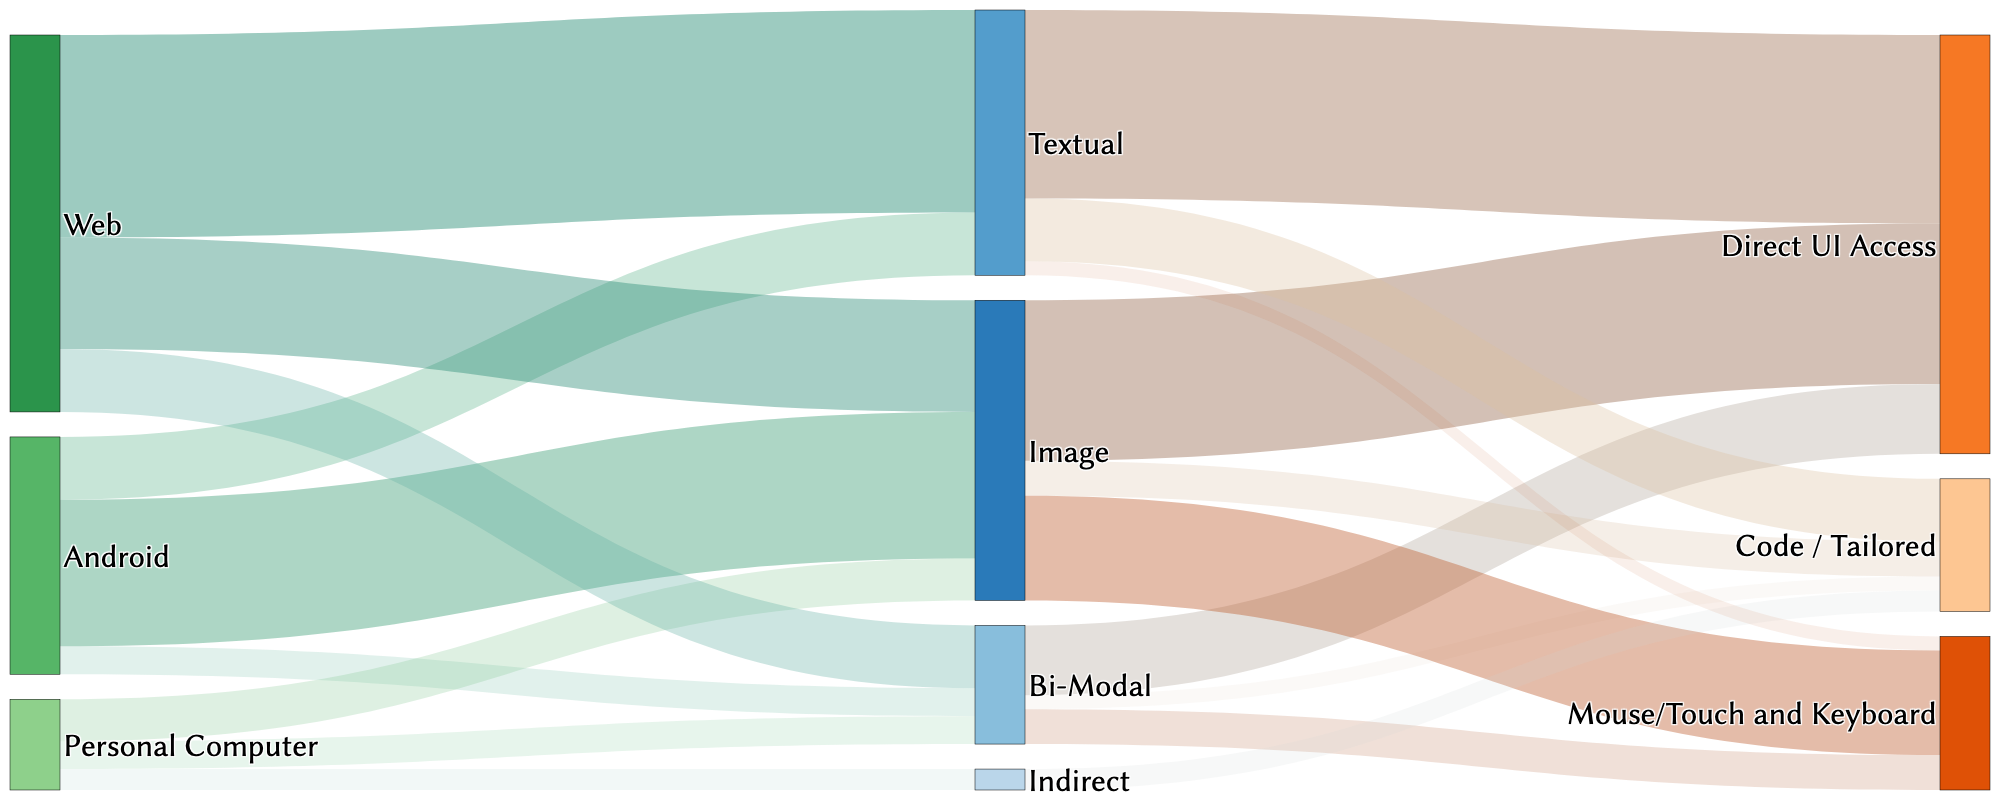
\includegraphics[width=1\linewidth]{figures/data/doa_sankey.png}
    \caption{Sankey diagram showing the connections between domains (left) and observation spaces (middle), and between observation and action spaces (right). The path width represents the number of papers within this survey associated with the corresponding topic.}
    \Description{A Sankey diagram with three columns depicting the relationships among surveyed research papers across domains, observation types, and action types. The left column enumerates the domains: Web, Android, and personal computer. The middle column presents observation types categorized as Image, textual, bi-modal, and indirect. The right column displays action types, including direct user interface (UI) access, mouse/touch and keyboard input, and code/tailored actions. Flows connect domains to observation types and subsequently to action types, with flow widths proportional to the number of papers associated with each connection. The strongest flows from domains to observations are from Web to textual data, Android to image, and Web to image. Among observation-to-action connections, the most prominent flows are from textual and image observations to direct UI access, with notable flows from image observations to mouse/touch and keyboard actions. This visualization provides a quantitative summary of prevailing research focuses within the surveyed literature.}
    \label{fig:domain-os-as-sankey}
\end{figure}


Different action types demand distinct observational inputs.
Coordinate-based actions (e.g., mouse clicks) depend on spatial information, whereas direct UI actions (e.g., button presses) must be able to reference UI elements. 
Consequently, coordinate-based actions naturally align with visual input, while element-based actions align with text-based input.

Nevertheless, our analysis shows many deviations from this expected alignment through modality bridging.
For instance, many vision-based agents employ direct UI access actions (see \cref{fig:domain-os-as-sankey}).
While such strategies can be effective, we argue that they are short-term workarounds tailored to existing technological constraints, introducing unnecessary long-term architectural complexity.

Historically, during the dominance of text-only LLMs, many ACUs converted screenshots into textual representations to maintain compatibility \citepeg{song_visiontasker_2024,wen_autodroid_2024}.  More recently, techniques such as set-of-mark prompting have been adopted to compensate for shortcomings in precise coordinate prediction \citepeg{zheng_gpt-4vision_2024,zhang_appagent_2023}.
These workarounds are likely to diminish in relevance as vision foundation models improve in spatial and semantic grounding.

Expanding on the premise that image-based observations offer a more coherent and spatially continuous representation of the user interface, we propose that \textbf{versatile ACUs should rely on mouse, touch, and keyboard actions} as these actions align naturally with visual observations.
Moreover, these actions can still be combined with higher-level subroutines (e.g., application switching) that abstract common interaction patterns into single actions.
